\documentclass[]{article}
\usepackage{lmodern}
\usepackage{amssymb,amsmath}
\usepackage{ifxetex,ifluatex}
\usepackage{fixltx2e} % provides \textsubscript
\ifnum 0\ifxetex 1\fi\ifluatex 1\fi=0 % if pdftex
  \usepackage[T1]{fontenc}
  \usepackage[utf8]{inputenc}
\else % if luatex or xelatex
  \ifxetex
    \usepackage{mathspec}
  \else
    \usepackage{fontspec}
  \fi
  \defaultfontfeatures{Ligatures=TeX,Scale=MatchLowercase}
\fi
% use upquote if available, for straight quotes in verbatim environments
\IfFileExists{upquote.sty}{\usepackage{upquote}}{}
% use microtype if available
\IfFileExists{microtype.sty}{%
\usepackage{microtype}
\UseMicrotypeSet[protrusion]{basicmath} % disable protrusion for tt fonts
}{}
\usepackage[margin=1in]{geometry}
\usepackage{hyperref}
\hypersetup{unicode=true,
            pdftitle={DS6050.FinalProject.Bender},
            pdfauthor={Alex Bender},
            pdfborder={0 0 0},
            breaklinks=true}
\urlstyle{same}  % don't use monospace font for urls
\usepackage{color}
\usepackage{fancyvrb}
\newcommand{\VerbBar}{|}
\newcommand{\VERB}{\Verb[commandchars=\\\{\}]}
\DefineVerbatimEnvironment{Highlighting}{Verbatim}{commandchars=\\\{\}}
% Add ',fontsize=\small' for more characters per line
\usepackage{framed}
\definecolor{shadecolor}{RGB}{248,248,248}
\newenvironment{Shaded}{\begin{snugshade}}{\end{snugshade}}
\newcommand{\AlertTok}[1]{\textcolor[rgb]{0.94,0.16,0.16}{#1}}
\newcommand{\AnnotationTok}[1]{\textcolor[rgb]{0.56,0.35,0.01}{\textbf{\textit{#1}}}}
\newcommand{\AttributeTok}[1]{\textcolor[rgb]{0.77,0.63,0.00}{#1}}
\newcommand{\BaseNTok}[1]{\textcolor[rgb]{0.00,0.00,0.81}{#1}}
\newcommand{\BuiltInTok}[1]{#1}
\newcommand{\CharTok}[1]{\textcolor[rgb]{0.31,0.60,0.02}{#1}}
\newcommand{\CommentTok}[1]{\textcolor[rgb]{0.56,0.35,0.01}{\textit{#1}}}
\newcommand{\CommentVarTok}[1]{\textcolor[rgb]{0.56,0.35,0.01}{\textbf{\textit{#1}}}}
\newcommand{\ConstantTok}[1]{\textcolor[rgb]{0.00,0.00,0.00}{#1}}
\newcommand{\ControlFlowTok}[1]{\textcolor[rgb]{0.13,0.29,0.53}{\textbf{#1}}}
\newcommand{\DataTypeTok}[1]{\textcolor[rgb]{0.13,0.29,0.53}{#1}}
\newcommand{\DecValTok}[1]{\textcolor[rgb]{0.00,0.00,0.81}{#1}}
\newcommand{\DocumentationTok}[1]{\textcolor[rgb]{0.56,0.35,0.01}{\textbf{\textit{#1}}}}
\newcommand{\ErrorTok}[1]{\textcolor[rgb]{0.64,0.00,0.00}{\textbf{#1}}}
\newcommand{\ExtensionTok}[1]{#1}
\newcommand{\FloatTok}[1]{\textcolor[rgb]{0.00,0.00,0.81}{#1}}
\newcommand{\FunctionTok}[1]{\textcolor[rgb]{0.00,0.00,0.00}{#1}}
\newcommand{\ImportTok}[1]{#1}
\newcommand{\InformationTok}[1]{\textcolor[rgb]{0.56,0.35,0.01}{\textbf{\textit{#1}}}}
\newcommand{\KeywordTok}[1]{\textcolor[rgb]{0.13,0.29,0.53}{\textbf{#1}}}
\newcommand{\NormalTok}[1]{#1}
\newcommand{\OperatorTok}[1]{\textcolor[rgb]{0.81,0.36,0.00}{\textbf{#1}}}
\newcommand{\OtherTok}[1]{\textcolor[rgb]{0.56,0.35,0.01}{#1}}
\newcommand{\PreprocessorTok}[1]{\textcolor[rgb]{0.56,0.35,0.01}{\textit{#1}}}
\newcommand{\RegionMarkerTok}[1]{#1}
\newcommand{\SpecialCharTok}[1]{\textcolor[rgb]{0.00,0.00,0.00}{#1}}
\newcommand{\SpecialStringTok}[1]{\textcolor[rgb]{0.31,0.60,0.02}{#1}}
\newcommand{\StringTok}[1]{\textcolor[rgb]{0.31,0.60,0.02}{#1}}
\newcommand{\VariableTok}[1]{\textcolor[rgb]{0.00,0.00,0.00}{#1}}
\newcommand{\VerbatimStringTok}[1]{\textcolor[rgb]{0.31,0.60,0.02}{#1}}
\newcommand{\WarningTok}[1]{\textcolor[rgb]{0.56,0.35,0.01}{\textbf{\textit{#1}}}}
\usepackage{graphicx,grffile}
\makeatletter
\def\maxwidth{\ifdim\Gin@nat@width>\linewidth\linewidth\else\Gin@nat@width\fi}
\def\maxheight{\ifdim\Gin@nat@height>\textheight\textheight\else\Gin@nat@height\fi}
\makeatother
% Scale images if necessary, so that they will not overflow the page
% margins by default, and it is still possible to overwrite the defaults
% using explicit options in \includegraphics[width, height, ...]{}
\setkeys{Gin}{width=\maxwidth,height=\maxheight,keepaspectratio}
\IfFileExists{parskip.sty}{%
\usepackage{parskip}
}{% else
\setlength{\parindent}{0pt}
\setlength{\parskip}{6pt plus 2pt minus 1pt}
}
\setlength{\emergencystretch}{3em}  % prevent overfull lines
\providecommand{\tightlist}{%
  \setlength{\itemsep}{0pt}\setlength{\parskip}{0pt}}
\setcounter{secnumdepth}{0}
% Redefines (sub)paragraphs to behave more like sections
\ifx\paragraph\undefined\else
\let\oldparagraph\paragraph
\renewcommand{\paragraph}[1]{\oldparagraph{#1}\mbox{}}
\fi
\ifx\subparagraph\undefined\else
\let\oldsubparagraph\subparagraph
\renewcommand{\subparagraph}[1]{\oldsubparagraph{#1}\mbox{}}
\fi

%%% Use protect on footnotes to avoid problems with footnotes in titles
\let\rmarkdownfootnote\footnote%
\def\footnote{\protect\rmarkdownfootnote}

%%% Change title format to be more compact
\usepackage{titling}

% Create subtitle command for use in maketitle
\providecommand{\subtitle}[1]{
  \posttitle{
    \begin{center}\large#1\end{center}
    }
}

\setlength{\droptitle}{-2em}

  \title{DS6050.FinalProject.Bender}
    \pretitle{\vspace{\droptitle}\centering\huge}
  \posttitle{\par}
    \author{Alex Bender}
    \preauthor{\centering\large\emph}
  \postauthor{\par}
      \predate{\centering\large\emph}
  \postdate{\par}
    \date{March 24, 2019}


\begin{document}
\maketitle

Data Description: Countries of the World - This data comes from the US
CIA. It is general characteristsics on different nations of the world.
Some columns included in the data are Region, Population, Area (sq.
mi.), Pop. Density (per sq. mi.), Coastline (coast/area ratio), Net
migration, Arable (\%), Crops (\%), Other (\%), Climate.

UN Human Development Data - This comes from the UN's 2015 Human
Development report, which was used to calculate the Human Development
Index. The datasets measures status of different nations in different
metrics of human development. Some columns included in the data are Life
Expectancy at Birth, Expected Years of Education, Mean Years of
Education, Gross National Income (GNI) per Capita, GNI per Capita Rank
Minus HDI Rank.

World Happiness - The World Happiness Report was released at the United
Nations at an event celebrating International Day of Happiness on March
20th. The report continues to gain global recognition. Happiness Score
is based on the World Happiness Report which includes GDP per Capita,
Family, Life Expectancy, Freedom, Generosity, Trust Government
Corruption, etc.

I am going to explore world happiness(WH), human development(HDI), and
country characteristics(CC) data in order to derive interesting
insights. I will be operating on the assumption of using the HDI data
from 2014, WH data from 2016, and CC data from as recent as 2017. Though
the data is not all from the same time period, I will be assuming that
the variation between the few years won't be significant enough to skew
results significantly.

\begin{Shaded}
\begin{Highlighting}[]
\CommentTok{#load country characteristics data}
\NormalTok{cc_data <-}\StringTok{ }\KeywordTok{read.csv}\NormalTok{(}\StringTok{"countries of the world.csv"}\NormalTok{, }\DataTypeTok{dec=}\StringTok{","}\NormalTok{)}

\CommentTok{#load 2016 world happiness data}
\NormalTok{wh2016 <-}\StringTok{ }\KeywordTok{read.csv}\NormalTok{(}\StringTok{"happiness2016.csv"}\NormalTok{)}

\CommentTok{#load 2014 HDI data}
\NormalTok{hdi2014 <-}\StringTok{ }\KeywordTok{read.csv}\NormalTok{(}\StringTok{"human_development.csv"}\NormalTok{, }\DataTypeTok{stringsAsFactors =} \OtherTok{FALSE}\NormalTok{)}
\end{Highlighting}
\end{Shaded}

\begin{Shaded}
\begin{Highlighting}[]
\CommentTok{#gather data understanding}
\KeywordTok{str}\NormalTok{(cc_data)}
\end{Highlighting}
\end{Shaded}

\begin{verbatim}
## 'data.frame':    227 obs. of  20 variables:
##  $ Country                           : Factor w/ 227 levels "Afghanistan ",..: 1 2 3 4 5 6 7 8 9 10 ...
##  $ Region                            : Factor w/ 11 levels "ASIA (EX. NEAR EAST)         ",..: 1 4 7 9 11 10 5 5 5 3 ...
##  $ Population                        : int  31056997 3581655 32930091 57794 71201 12127071 13477 69108 39921833 2976372 ...
##  $ Area..sq..mi..                    : int  647500 28748 2381740 199 468 1246700 102 443 2766890 29800 ...
##  $ Pop..Density..per.sq..mi..        : num  48 124.6 13.8 290.4 152.1 ...
##  $ Coastline..coast.area.ratio.      : num  0 1.26 0.04 58.29 0 ...
##  $ Net.migration                     : num  23.06 -4.93 -0.39 -20.71 6.6 ...
##  $ Infant.mortality..per.1000.births.: num  163.07 21.52 31 9.27 4.05 ...
##  $ GDP....per.capita.                : int  700 4500 6000 8000 19000 1900 8600 11000 11200 3500 ...
##  $ Literacy....                      : num  36 86.5 70 97 100 42 95 89 97.1 98.6 ...
##  $ Phones..per.1000.                 : num  3.2 71.2 78.1 259.5 497.2 ...
##  $ Arable....                        : num  12.13 21.09 3.22 10 2.22 ...
##  $ Crops....                         : num  0.22 4.42 0.25 15 0 0.24 0 4.55 0.48 2.3 ...
##  $ Other....                         : num  87.7 74.5 96.5 75 97.8 ...
##  $ Climate                           : num  1 3 1 2 3 NA 2 2 3 4 ...
##  $ Birthrate                         : num  46.6 15.11 17.14 22.46 8.71 ...
##  $ Deathrate                         : num  20.34 5.22 4.61 3.27 6.25 ...
##  $ Agriculture                       : num  0.38 0.232 0.101 NA NA 0.096 0.04 0.038 0.095 0.239 ...
##  $ Industry                          : num  0.24 0.188 0.6 NA NA 0.658 0.18 0.22 0.358 0.343 ...
##  $ Service                           : num  0.38 0.579 0.298 NA NA 0.246 0.78 0.743 0.547 0.418 ...
\end{verbatim}

\begin{Shaded}
\begin{Highlighting}[]
\KeywordTok{summary}\NormalTok{(cc_data)}
\end{Highlighting}
\end{Shaded}

\begin{verbatim}
##             Country                                    Region  
##  Afghanistan    :  1   SUB-SAHARAN AFRICA                 :51  
##  Albania        :  1   LATIN AMER. & CARIB                :45  
##  Algeria        :  1   ASIA (EX. NEAR EAST)               :28  
##  American Samoa :  1   WESTERN EUROPE                     :28  
##  Andorra        :  1   OCEANIA                            :21  
##  Angola         :  1   NEAR EAST                          :16  
##  (Other)        :221   (Other)                            :38  
##    Population        Area..sq..mi..     Pop..Density..per.sq..mi..
##  Min.   :7.026e+03   Min.   :       2   Min.   :    0.00          
##  1st Qu.:4.376e+05   1st Qu.:    4648   1st Qu.:   29.15          
##  Median :4.787e+06   Median :   86600   Median :   78.80          
##  Mean   :2.874e+07   Mean   :  598227   Mean   :  379.05          
##  3rd Qu.:1.750e+07   3rd Qu.:  441811   3rd Qu.:  190.15          
##  Max.   :1.314e+09   Max.   :17075200   Max.   :16271.50          
##                                                                   
##  Coastline..coast.area.ratio. Net.migration      
##  Min.   :  0.00               Min.   :-20.99000  
##  1st Qu.:  0.10               1st Qu.: -0.92750  
##  Median :  0.73               Median :  0.00000  
##  Mean   : 21.17               Mean   :  0.03812  
##  3rd Qu.: 10.35               3rd Qu.:  0.99750  
##  Max.   :870.66               Max.   : 23.06000  
##                               NA's   :3          
##  Infant.mortality..per.1000.births. GDP....per.capita.  Literacy....   
##  Min.   :  2.29                     Min.   :  500      Min.   : 17.60  
##  1st Qu.:  8.15                     1st Qu.: 1900      1st Qu.: 70.60  
##  Median : 21.00                     Median : 5550      Median : 92.50  
##  Mean   : 35.51                     Mean   : 9690      Mean   : 82.84  
##  3rd Qu.: 55.70                     3rd Qu.:15700      3rd Qu.: 98.00  
##  Max.   :191.19                     Max.   :55100      Max.   :100.00  
##  NA's   :3                          NA's   :1          NA's   :18      
##  Phones..per.1000.   Arable....      Crops....        Other....     
##  Min.   :   0.2    Min.   : 0.00   Min.   : 0.000   Min.   : 33.33  
##  1st Qu.:  37.8    1st Qu.: 3.22   1st Qu.: 0.190   1st Qu.: 71.65  
##  Median : 176.2    Median :10.42   Median : 1.030   Median : 85.70  
##  Mean   : 236.1    Mean   :13.80   Mean   : 4.564   Mean   : 81.64  
##  3rd Qu.: 389.6    3rd Qu.:20.00   3rd Qu.: 4.440   3rd Qu.: 95.44  
##  Max.   :1035.6    Max.   :62.11   Max.   :50.680   Max.   :100.00  
##  NA's   :4         NA's   :2       NA's   :2        NA's   :2       
##     Climate        Birthrate       Deathrate       Agriculture     
##  Min.   :1.000   Min.   : 7.29   Min.   : 2.290   Min.   :0.00000  
##  1st Qu.:2.000   1st Qu.:12.67   1st Qu.: 5.910   1st Qu.:0.03775  
##  Median :2.000   Median :18.79   Median : 7.840   Median :0.09900  
##  Mean   :2.139   Mean   :22.11   Mean   : 9.241   Mean   :0.15084  
##  3rd Qu.:3.000   3rd Qu.:29.82   3rd Qu.:10.605   3rd Qu.:0.22100  
##  Max.   :4.000   Max.   :50.73   Max.   :29.740   Max.   :0.76900  
##  NA's   :22      NA's   :3       NA's   :4        NA's   :15       
##     Industry         Service      
##  Min.   :0.0200   Min.   :0.0620  
##  1st Qu.:0.1930   1st Qu.:0.4293  
##  Median :0.2720   Median :0.5710  
##  Mean   :0.2827   Mean   :0.5653  
##  3rd Qu.:0.3410   3rd Qu.:0.6785  
##  Max.   :0.9060   Max.   :0.9540  
##  NA's   :16       NA's   :15
\end{verbatim}

\begin{Shaded}
\begin{Highlighting}[]
\KeywordTok{head}\NormalTok{(cc_data)}
\end{Highlighting}
\end{Shaded}

\begin{verbatim}
##           Country                              Region Population
## 1    Afghanistan        ASIA (EX. NEAR EAST)            31056997
## 2        Albania  EASTERN EUROPE                         3581655
## 3        Algeria  NORTHERN AFRICA                       32930091
## 4 American Samoa  OCEANIA                                  57794
## 5        Andorra  WESTERN EUROPE                           71201
## 6         Angola  SUB-SAHARAN AFRICA                    12127071
##   Area..sq..mi.. Pop..Density..per.sq..mi.. Coastline..coast.area.ratio.
## 1         647500                       48.0                         0.00
## 2          28748                      124.6                         1.26
## 3        2381740                       13.8                         0.04
## 4            199                      290.4                        58.29
## 5            468                      152.1                         0.00
## 6        1246700                        9.7                         0.13
##   Net.migration Infant.mortality..per.1000.births. GDP....per.capita.
## 1         23.06                             163.07                700
## 2         -4.93                              21.52               4500
## 3         -0.39                              31.00               6000
## 4        -20.71                               9.27               8000
## 5          6.60                               4.05              19000
## 6          0.00                             191.19               1900
##   Literacy.... Phones..per.1000. Arable.... Crops.... Other.... Climate
## 1         36.0               3.2      12.13      0.22     87.65       1
## 2         86.5              71.2      21.09      4.42     74.49       3
## 3         70.0              78.1       3.22      0.25     96.53       1
## 4         97.0             259.5      10.00     15.00     75.00       2
## 5        100.0             497.2       2.22      0.00     97.78       3
## 6         42.0               7.8       2.41      0.24     97.35      NA
##   Birthrate Deathrate Agriculture Industry Service
## 1     46.60     20.34       0.380    0.240   0.380
## 2     15.11      5.22       0.232    0.188   0.579
## 3     17.14      4.61       0.101    0.600   0.298
## 4     22.46      3.27          NA       NA      NA
## 5      8.71      6.25          NA       NA      NA
## 6     45.11     24.20       0.096    0.658   0.246
\end{verbatim}

\begin{Shaded}
\begin{Highlighting}[]
\CommentTok{#gather data understanding}
\KeywordTok{str}\NormalTok{(hdi2014)}
\end{Highlighting}
\end{Shaded}

\begin{verbatim}
## 'data.frame':    195 obs. of  8 variables:
##  $ HDI.Rank                              : int  1 2 3 4 5 6 6 8 9 9 ...
##  $ Country                               : chr  "Norway" "Australia" "Switzerland" "Denmark" ...
##  $ Human.Development.Index..HDI.         : num  0.944 0.935 0.93 0.923 0.922 0.916 0.916 0.915 0.913 0.913 ...
##  $ Life.Expectancy.at.Birth              : num  81.6 82.4 83 80.2 81.6 80.9 80.9 79.1 82 81.8 ...
##  $ Expected.Years.of.Education           : num  17.5 20.2 15.8 18.7 17.9 16.5 18.6 16.5 15.9 19.2 ...
##  $ Mean.Years.of.Education               : num  12.6 13 12.8 12.7 11.9 13.1 12.2 12.9 13 12.5 ...
##  $ Gross.National.Income..GNI..per.Capita: chr  "64,992" "42,261" "56,431" "44,025" ...
##  $ GNI.per.Capita.Rank.Minus.HDI.Rank    : int  5 17 6 11 9 11 16 3 11 23 ...
\end{verbatim}

\begin{Shaded}
\begin{Highlighting}[]
\KeywordTok{summary}\NormalTok{(hdi2014)}
\end{Highlighting}
\end{Shaded}

\begin{verbatim}
##     HDI.Rank        Country          Human.Development.Index..HDI.
##  Min.   :  1.00   Length:195         Min.   :0.3480               
##  1st Qu.: 47.75   Class :character   1st Qu.:0.5770               
##  Median : 94.00   Mode  :character   Median :0.7210               
##  Mean   : 94.31                      Mean   :0.6918               
##  3rd Qu.:141.25                      3rd Qu.:0.8000               
##  Max.   :188.00                      Max.   :0.9440               
##  NA's   :7                                                        
##  Life.Expectancy.at.Birth Expected.Years.of.Education
##  Min.   :49.00            Min.   : 4.10              
##  1st Qu.:65.75            1st Qu.:11.10              
##  Median :73.10            Median :13.10              
##  Mean   :71.07            Mean   :12.86              
##  3rd Qu.:76.80            3rd Qu.:14.90              
##  Max.   :84.00            Max.   :20.20              
##                                                      
##  Mean.Years.of.Education Gross.National.Income..GNI..per.Capita
##  Min.   : 1.400          Length:195                            
##  1st Qu.: 5.550          Class :character                      
##  Median : 8.400          Mode  :character                      
##  Mean   : 8.079                                                
##  3rd Qu.:10.600                                                
##  Max.   :13.100                                                
##                                                                
##  GNI.per.Capita.Rank.Minus.HDI.Rank
##  Min.   :-84.0000                  
##  1st Qu.: -9.0000                  
##  Median :  1.5000                  
##  Mean   :  0.1862                  
##  3rd Qu.: 11.0000                  
##  Max.   : 47.0000                  
##  NA's   :7
\end{verbatim}

\begin{Shaded}
\begin{Highlighting}[]
\KeywordTok{head}\NormalTok{(hdi2014)}
\end{Highlighting}
\end{Shaded}

\begin{verbatim}
##   HDI.Rank     Country Human.Development.Index..HDI.
## 1        1      Norway                         0.944
## 2        2   Australia                         0.935
## 3        3 Switzerland                         0.930
## 4        4     Denmark                         0.923
## 5        5 Netherlands                         0.922
## 6        6     Germany                         0.916
##   Life.Expectancy.at.Birth Expected.Years.of.Education
## 1                     81.6                        17.5
## 2                     82.4                        20.2
## 3                     83.0                        15.8
## 4                     80.2                        18.7
## 5                     81.6                        17.9
## 6                     80.9                        16.5
##   Mean.Years.of.Education Gross.National.Income..GNI..per.Capita
## 1                    12.6                                 64,992
## 2                    13.0                                 42,261
## 3                    12.8                                 56,431
## 4                    12.7                                 44,025
## 5                    11.9                                 45,435
## 6                    13.1                                 43,919
##   GNI.per.Capita.Rank.Minus.HDI.Rank
## 1                                  5
## 2                                 17
## 3                                  6
## 4                                 11
## 5                                  9
## 6                                 11
\end{verbatim}

\begin{Shaded}
\begin{Highlighting}[]
\CommentTok{#gather data understanding}
\KeywordTok{str}\NormalTok{(wh2016)}
\end{Highlighting}
\end{Shaded}

\begin{verbatim}
## 'data.frame':    157 obs. of  13 variables:
##  $ Country                      : Factor w/ 157 levels "Afghanistan",..: 38 135 58 104 45 26 98 99 7 134 ...
##  $ Region                       : Factor w/ 10 levels "Australia and New Zealand",..: 10 10 10 10 10 6 10 1 1 10 ...
##  $ Happiness.Rank               : int  1 2 3 4 5 6 7 8 9 10 ...
##  $ Happiness.Score              : num  7.53 7.51 7.5 7.5 7.41 ...
##  $ Lower.Confidence.Interval    : num  7.46 7.43 7.33 7.42 7.35 ...
##  $ Upper.Confidence.Interval    : num  7.59 7.59 7.67 7.58 7.47 ...
##  $ Economy..GDP.per.Capita.     : num  1.44 1.53 1.43 1.58 1.41 ...
##  $ Family                       : num  1.16 1.15 1.18 1.13 1.13 ...
##  $ Health..Life.Expectancy.     : num  0.795 0.863 0.867 0.796 0.811 ...
##  $ Freedom                      : num  0.579 0.586 0.566 0.596 0.571 ...
##  $ Trust..Government.Corruption.: num  0.445 0.412 0.15 0.358 0.41 ...
##  $ Generosity                   : num  0.362 0.281 0.477 0.379 0.255 ...
##  $ Dystopia.Residual            : num  2.74 2.69 2.83 2.66 2.83 ...
\end{verbatim}

\begin{Shaded}
\begin{Highlighting}[]
\KeywordTok{summary}\NormalTok{(wh2016)}
\end{Highlighting}
\end{Shaded}

\begin{verbatim}
##         Country                                Region   Happiness.Rank  
##  Afghanistan:  1   Sub-Saharan Africa             :38   Min.   :  1.00  
##  Albania    :  1   Central and Eastern Europe     :29   1st Qu.: 40.00  
##  Algeria    :  1   Latin America and Caribbean    :24   Median : 79.00  
##  Angola     :  1   Western Europe                 :21   Mean   : 78.98  
##  Argentina  :  1   Middle East and Northern Africa:19   3rd Qu.:118.00  
##  Armenia    :  1   Southeastern Asia              : 9   Max.   :157.00  
##  (Other)    :151   (Other)                        :17                   
##  Happiness.Score Lower.Confidence.Interval Upper.Confidence.Interval
##  Min.   :2.905   Min.   :2.732             Min.   :3.078            
##  1st Qu.:4.404   1st Qu.:4.327             1st Qu.:4.465            
##  Median :5.314   Median :5.237             Median :5.419            
##  Mean   :5.382   Mean   :5.282             Mean   :5.482            
##  3rd Qu.:6.269   3rd Qu.:6.154             3rd Qu.:6.434            
##  Max.   :7.526   Max.   :7.460             Max.   :7.669            
##                                                                     
##  Economy..GDP.per.Capita.     Family       Health..Life.Expectancy.
##  Min.   :0.0000           Min.   :0.0000   Min.   :0.0000          
##  1st Qu.:0.6702           1st Qu.:0.6418   1st Qu.:0.3829          
##  Median :1.0278           Median :0.8414   Median :0.5966          
##  Mean   :0.9539           Mean   :0.7936   Mean   :0.5576          
##  3rd Qu.:1.2796           3rd Qu.:1.0215   3rd Qu.:0.7299          
##  Max.   :1.8243           Max.   :1.1833   Max.   :0.9528          
##                                                                    
##     Freedom       Trust..Government.Corruption.   Generosity    
##  Min.   :0.0000   Min.   :0.00000               Min.   :0.0000  
##  1st Qu.:0.2575   1st Qu.:0.06126               1st Qu.:0.1546  
##  Median :0.3975   Median :0.10547               Median :0.2225  
##  Mean   :0.3710   Mean   :0.13762               Mean   :0.2426  
##  3rd Qu.:0.4845   3rd Qu.:0.17554               3rd Qu.:0.3119  
##  Max.   :0.6085   Max.   :0.50521               Max.   :0.8197  
##                                                                 
##  Dystopia.Residual
##  Min.   :0.8179   
##  1st Qu.:2.0317   
##  Median :2.2907   
##  Mean   :2.3258   
##  3rd Qu.:2.6646   
##  Max.   :3.8377   
## 
\end{verbatim}

\begin{Shaded}
\begin{Highlighting}[]
\KeywordTok{head}\NormalTok{(wh2016)}
\end{Highlighting}
\end{Shaded}

\begin{verbatim}
##       Country         Region Happiness.Rank Happiness.Score
## 1     Denmark Western Europe              1           7.526
## 2 Switzerland Western Europe              2           7.509
## 3     Iceland Western Europe              3           7.501
## 4      Norway Western Europe              4           7.498
## 5     Finland Western Europe              5           7.413
## 6      Canada  North America              6           7.404
##   Lower.Confidence.Interval Upper.Confidence.Interval
## 1                     7.460                     7.592
## 2                     7.428                     7.590
## 3                     7.333                     7.669
## 4                     7.421                     7.575
## 5                     7.351                     7.475
## 6                     7.335                     7.473
##   Economy..GDP.per.Capita.  Family Health..Life.Expectancy. Freedom
## 1                  1.44178 1.16374                  0.79504 0.57941
## 2                  1.52733 1.14524                  0.86303 0.58557
## 3                  1.42666 1.18326                  0.86733 0.56624
## 4                  1.57744 1.12690                  0.79579 0.59609
## 5                  1.40598 1.13464                  0.81091 0.57104
## 6                  1.44015 1.09610                  0.82760 0.57370
##   Trust..Government.Corruption. Generosity Dystopia.Residual
## 1                       0.44453    0.36171           2.73939
## 2                       0.41203    0.28083           2.69463
## 3                       0.14975    0.47678           2.83137
## 4                       0.35776    0.37895           2.66465
## 5                       0.41004    0.25492           2.82596
## 6                       0.31329    0.44834           2.70485
\end{verbatim}

As you can see all of the loaded data has different numbers of rows,
meaning that different countries are included in the different datasets.
This will be reconcilied by only including the countries located in the
dataset with the least amount of countries (world happiness 2016). Since
my analysis relies on merging the unqiue nation metrics from the various
datasets, it would be wise to only included the countries with full
data. Still, this leaves us with over 150 countries, which is enough to
run both numeric prediction (regression) and classification data mining
tasks.The data set is a similar size to the built in Iris dataset, with
more dimensions, so it should still be fine. I will combat this small
amount of data with the use of k-fold Cross-validation.

My plan of attack: - I am going to use the 2016 World Happiness data as
my basis for dependent variables. - I plan to do numeric
prediction/regression by predicting the happiness score of a nation
using the happiness score column from the wh2016 data. I will be
exploring multiple linear regression, regression tree, neural network,
and kNN models. - As my independent variables I will be using the Human
Development Index and Country Characteristics data in order to attempt
to predict the target/response variables from the world happiness data.
- I won't be using the additional features in the World Happiness data
as predictors for two reasons. 1) The world happiness score is a direct
calculation from these features, so I don't want to risk overfitting by
the model just memorizing the calculation essentially. 2) I want to
derive novel insights from a various set of predictors from the other
two datasets.

If I have time: - Classification for region of the world based on the
features - Derive an attribute that is a binary indicator of happy or
not in order to do binary classification using SVM and/or Logistic
regression.

Now we have to merge the datasets properly. First we have to match up
the rows based on Country name. If different datasets name countries
differently, this will pose a challenge.

\begin{Shaded}
\begin{Highlighting}[]
\KeywordTok{library}\NormalTok{(tidyverse)}
\end{Highlighting}
\end{Shaded}

\begin{verbatim}
## -- Attaching packages ----------------------------------------------------------------------------------------------------- tidyverse 1.2.1 --
\end{verbatim}

\begin{verbatim}
## v ggplot2 3.1.0       v purrr   0.3.2  
## v tibble  2.1.1       v dplyr   0.8.0.1
## v tidyr   0.8.3       v stringr 1.4.0  
## v readr   1.3.1       v forcats 0.4.0
\end{verbatim}

\begin{verbatim}
## -- Conflicts -------------------------------------------------------------------------------------------------------- tidyverse_conflicts() --
## x dplyr::filter() masks stats::filter()
## x dplyr::lag()    masks stats::lag()
\end{verbatim}

To reduce chances for errors down the line, let's trim any additional
whitespaces from the data.

\begin{Shaded}
\begin{Highlighting}[]
\CommentTok{#Get rid of unnecessary whitespace}
\NormalTok{cc_data}\OperatorTok{$}\NormalTok{Country <-}\StringTok{ }\KeywordTok{str_trim}\NormalTok{(cc_data}\OperatorTok{$}\NormalTok{Country) }\OperatorTok\StringTok{ }\KeywordTok{as.factor}\NormalTok{()}
\NormalTok{cc_data}\OperatorTok{$}\NormalTok{Region <-}\StringTok{ }\KeywordTok{str_trim}\NormalTok{(cc_data}\OperatorTok{$}\NormalTok{Region) }\OperatorTok\StringTok{ }\KeywordTok{as.factor}\NormalTok{()}
\NormalTok{hdi2014}\OperatorTok{$}\NormalTok{Country <-}\StringTok{ }\KeywordTok{str_trim}\NormalTok{(hdi2014}\OperatorTok{$}\NormalTok{Country) }\OperatorTok\StringTok{ }\KeywordTok{as.factor}\NormalTok{()}
\NormalTok{wh2016}\OperatorTok{$}\NormalTok{Country <-}\StringTok{ }\KeywordTok{str_trim}\NormalTok{(wh2016}\OperatorTok{$}\NormalTok{Country) }\OperatorTok\StringTok{ }\KeywordTok{as.factor}\NormalTok{()}
\NormalTok{wh2016}\OperatorTok{$}\NormalTok{Region <-}\StringTok{ }\KeywordTok{str_trim}\NormalTok{(wh2016}\OperatorTok{$}\NormalTok{Region) }\OperatorTok\StringTok{ }\KeywordTok{as.factor}\NormalTok{()}
\end{Highlighting}
\end{Shaded}

Let's only select the two target/response variables and the country from
the world happiness data.

\begin{Shaded}
\begin{Highlighting}[]
\CommentTok{#select only the needed columns }
\NormalTok{wh2016 <-}\StringTok{ }\KeywordTok{select}\NormalTok{(wh2016, Country, Region, Happiness.Score)}
\end{Highlighting}
\end{Shaded}

We know from this dataset that we will be looking at 157 countries.

I am going to standardize all of the country names using a convenient
function in the standardize text package. The function recognizes common
variations of country names and essentially ``Autocorrects'' them into a
standard format. This will help a lot when joining datasets together.

\begin{Shaded}
\begin{Highlighting}[]
\CommentTok{#install.packages("StandardizeText")}
\KeywordTok{library}\NormalTok{(StandardizeText)}

\CommentTok{#Standardize column using default country names}
\NormalTok{hdi2014}\OperatorTok{$}\NormalTok{Country <-}\StringTok{ }\KeywordTok{standardize.countrynames}\NormalTok{(hdi2014}\OperatorTok{$}\NormalTok{Country,}\DataTypeTok{suggest=}\StringTok{"auto"}\NormalTok{, }\DataTypeTok{verbose =}\NormalTok{ T)}
\end{Highlighting}
\end{Shaded}

\begin{verbatim}
## 
## The following names were not recoginized and left unchanged:
## [1] "Arab States"                     "Côte d'Ivoire"                 
## [3] "Cabo Verde"                      "East Asia and the Pacific"      
## [5] "Europe and Central Asia"         "Latin America and the Caribbean"
## [7] "South Asia"                      "Sub-Saharan Africa"             
## 
## The following names were changed:
##                                     Original
## 1           Bolivia (Plurinational State of)
## 2                                      Congo
## 3         Congo (Democratic Republic of the)
## 4                 Iran (Islamic Republic of)
## 5                        Korea (Republic of)
## 6           Lao People's Democratic Republic
## 7           Micronesia (Federated States of)
## 8                      Moldova (Republic of)
## 9                        Palestine, State of
## 10                     Saint Kitts and Nevis
## 11                               Saint Lucia
## 12          Saint Vincent and the Grenadines
## 13                                  Slovakia
## 14             Tanzania (United Republic of)
## 15 The former Yugoslav Republic of Macedonia
## 16        Venezuela (Bolivarian Republic of)
## 17                                  Viet Nam
##                          Modified
## 1                         Bolivia
## 2                  Congo Republic
## 3       Congo Democratic Republic
## 4                            Iran
## 5                  Korea Republic
## 6                            Laos
## 7                      Micronesia
## 8                         Moldova
## 9           Palestinian Territory
## 10            St. Kitts and Nevis
## 11                      St. Lucia
## 12 St. Vincent and the Grenadines
## 13                Slovak Republic
## 14                       Tanzania
## 15                      Macedonia
## 16                      Venezuela
## 17                        Vietnam
## 
## The following suggested changes were applied:
##                 Original Suggested
## 1 Hong Kong, China (SAR) Hong Kong
\end{verbatim}

I can see here that some useful changes were made! Also it seems there
was an encoding error for ``Côte d'Ivoire'', so I will manually change
this to ``Cote d'Ivoire'' in the hdi2014 dataset.

\begin{Shaded}
\begin{Highlighting}[]
\CommentTok{#Replace mistake manually}
\NormalTok{hdi2014}\OperatorTok{$}\NormalTok{Country[}\KeywordTok{which}\NormalTok{(hdi2014}\OperatorTok{$}\NormalTok{Country}\OperatorTok{==}\StringTok{"Côte d'Ivoire"}\NormalTok{)] <-}\StringTok{ "Cote d'Ivoire"}

\CommentTok{#Make sure it worked}
\NormalTok{hdi2014}\OperatorTok{$}\NormalTok{Country[}\KeywordTok{which}\NormalTok{(hdi2014}\OperatorTok{$}\NormalTok{Country}\OperatorTok{==}\StringTok{"Côte d'Ivoire"}\NormalTok{)]}
\end{Highlighting}
\end{Shaded}

\begin{verbatim}
## character(0)
\end{verbatim}

\begin{Shaded}
\begin{Highlighting}[]
\NormalTok{hdi2014}\OperatorTok{$}\NormalTok{Country[}\KeywordTok{which}\NormalTok{(hdi2014}\OperatorTok{$}\NormalTok{Country}\OperatorTok{==}\StringTok{"Cote d'Ivoire"}\NormalTok{)]}
\end{Highlighting}
\end{Shaded}

\begin{verbatim}
## [1] "Cote d'Ivoire"
\end{verbatim}

\begin{Shaded}
\begin{Highlighting}[]
\CommentTok{#Standardize column using default country names}
\NormalTok{wh2016}\OperatorTok{$}\NormalTok{Country <-}\StringTok{ }\KeywordTok{standardize.countrynames}\NormalTok{(wh2016}\OperatorTok{$}\NormalTok{Country,}\DataTypeTok{suggest=}\StringTok{"auto"}\NormalTok{, }\DataTypeTok{verbose =}\NormalTok{ T)}
\end{Highlighting}
\end{Shaded}

\begin{verbatim}
## 
## The following names were not recoginized and left unchanged:
## [1] "North Cyprus"      "Somaliland Region"
## 
## The following names were changed:
##                  Original                  Modified
## 1     Congo (Brazzaville)            Congo Republic
## 2        Congo (Kinshasa) Congo Democratic Republic
## 3             Ivory Coast             Cote d'Ivoire
## 4 Palestinian Territories     Palestinian Territory
## 5                  Russia        Russian Federation
## 6                Slovakia           Slovak Republic
## 7             South Korea            Korea Republic
## 8                   Syria      Syrian Arab Republic
\end{verbatim}

This data had 8 names that required standardization! Also, some names
weren't recognized, but we will see if we need those.

\begin{Shaded}
\begin{Highlighting}[]
\CommentTok{#Standardize column using default country names}
\NormalTok{cc_data}\OperatorTok{$}\NormalTok{Country <-}\StringTok{ }\KeywordTok{standardize.countrynames}\NormalTok{(cc_data}\OperatorTok{$}\NormalTok{Country,}\DataTypeTok{suggest=}\StringTok{"auto"}\NormalTok{)}
\end{Highlighting}
\end{Shaded}

\begin{verbatim}
## 
## Note: 3 names were not recoginized and left unchanged.
## 
## The following names were changed:
##                            Original                       Modified
## 1                 Antigua & Barbuda            Antigua and Barbuda
## 2                      Bahamas, The                        Bahamas
## 3              Bosnia & Herzegovina         Bosnia and Herzegovina
## 4                British Virgin Is.              Virgin Islands BR
## 5                            Brunei              Brunei Darussalam
## 6              Central African Rep.       Central African Republic
## 7                  Congo, Dem. Rep.      Congo Democratic Republic
## 8                        East Timor                    Timor-Leste
## 9                       Gambia, The                         Gambia
## 10                     Korea, North      Korea Democratic Republic
## 11                     Korea, South                 Korea Republic
## 12                            Macau                          Macao
## 13                           Russia             Russian Federation
## 14                     Saint Helena                     St. Helena
## 15              Saint Kitts & Nevis            St. Kitts and Nevis
## 16                      Saint Lucia                      St. Lucia
## 17 Saint Vincent and the Grenadines St. Vincent and the Grenadines
## 18              Sao Tome & Principe          Sao Tome and Principe
## 19                         Slovakia                Slovak Republic
## 20             St Pierre & Miquelon        St. Pierre and Miquelon
## 21                            Syria           Syrian Arab Republic
## 22                Trinidad & Tobago            Trinidad and Tobago
## 23                Turks & Caicos Is       Turks and Caicos Islands
## 
## The following suggested changes were applied:
##               Original      Suggested
## 1 Congo, Repub. of the Congo Republic
## 2 Micronesia, Fed. St.     Micronesia
\end{verbatim}

Perfect! Now all country names should be standardized, so we can do a
join.Let's see which countries from the world happiness data do not have
a match in the human development data using an anti-join.

\begin{Shaded}
\begin{Highlighting}[]
\CommentTok{#make sure the country name standardization worked}
\NormalTok{non_matches <-}\StringTok{ }\KeywordTok{anti_join}\NormalTok{(wh2016[}\DecValTok{1}\NormalTok{], hdi2014[}\DecValTok{2}\NormalTok{], }\DataTypeTok{by =} \StringTok{"Country"}\NormalTok{)}
\NormalTok{non_matches2 <-}\StringTok{ }\KeywordTok{anti_join}\NormalTok{(wh2016[}\DecValTok{1}\NormalTok{], cc_data[}\DecValTok{1}\NormalTok{] , }\DataTypeTok{by =} \StringTok{"Country"}\NormalTok{)}

\CommentTok{#print out distinct non-matches}
\KeywordTok{distinct}\NormalTok{(}\KeywordTok{rbind}\NormalTok{(non_matches,non_matches2))}
\end{Highlighting}
\end{Shaded}

\begin{verbatim}
##                  Country
## 1            Puerto Rico
## 2                 Taiwan
## 3           North Cyprus
## 4                Somalia
## 5                 Kosovo
## 6      Somaliland Region
## 7             Montenegro
## 8  Palestinian Territory
## 9                Myanmar
## 10           South Sudan
\end{verbatim}

The countries that have a happiness score but do not have any data in
either the HDI data or the CC data are Puerto Rico, Taiwan, North
Cyprus, Somalia, Kosovo, Somaliland Region, Montenegro, Palestinian
Territory, Myanmar, and South Sudan. Because these countries don't have
any data from the other datasets for the dependent/response/target
variable, they would essentially be complete empty rows. From the
eventual merged data, I will be removing these countries for the
analysis. This will leave us with 147 countries to analyze, which is
still enough to draw meaningful insights.

In order to merge the datasets, I am going to do an inner join, which
will essentially pull all the data that both datasets have based on
matching the ``Country'' column. For example, a sample row will contain
the data columns located in the all three datasets for a single country
name, such as France.

\begin{Shaded}
\begin{Highlighting}[]
\CommentTok{#merge datasets to make final dataset}
\NormalTok{world_df <-}\StringTok{ }\KeywordTok{inner_join}\NormalTok{(wh2016, hdi2014, }\DataTypeTok{by =} \StringTok{"Country"}\NormalTok{)}

\NormalTok{world_df <-}\StringTok{ }\KeywordTok{inner_join}\NormalTok{(world_df, cc_data, }\DataTypeTok{by =} \StringTok{"Country"}\NormalTok{)}

\KeywordTok{nrow}\NormalTok{(world_df)}
\end{Highlighting}
\end{Shaded}

\begin{verbatim}
## [1] 147
\end{verbatim}

147 countries remaining, perfect!

Let's make sure the join worked correctly by spot checking a country

\begin{Shaded}
\begin{Highlighting}[]
\NormalTok{cc_data[}\KeywordTok{which}\NormalTok{(cc_data}\OperatorTok{$}\NormalTok{Country}\OperatorTok{==}\StringTok{"France"}\NormalTok{),}\StringTok{"Population"}\NormalTok{]}
\end{Highlighting}
\end{Shaded}

\begin{verbatim}
## [1] 60876136
\end{verbatim}

\begin{Shaded}
\begin{Highlighting}[]
\NormalTok{hdi2014[}\KeywordTok{which}\NormalTok{(hdi2014}\OperatorTok{$}\NormalTok{Country}\OperatorTok{==}\StringTok{"France"}\NormalTok{),}\StringTok{"Mean.Years.of.Education"}\NormalTok{]}
\end{Highlighting}
\end{Shaded}

\begin{verbatim}
## [1] 11.1
\end{verbatim}

\begin{Shaded}
\begin{Highlighting}[]
\NormalTok{wh2016[}\KeywordTok{which}\NormalTok{(wh2016}\OperatorTok{$}\NormalTok{Country}\OperatorTok{==}\StringTok{"France"}\NormalTok{),}\StringTok{"Happiness.Score"}\NormalTok{]}
\end{Highlighting}
\end{Shaded}

\begin{verbatim}
## [1] 6.478
\end{verbatim}

\begin{Shaded}
\begin{Highlighting}[]
\NormalTok{world_df[}\KeywordTok{which}\NormalTok{(world_df}\OperatorTok{$}\NormalTok{Country}\OperatorTok{==}\StringTok{"France"}\NormalTok{),}\KeywordTok{c}\NormalTok{(}\StringTok{"Population"}\NormalTok{, }\StringTok{"Mean.Years.of.Education"}\NormalTok{, }\StringTok{"Happiness.Score"}\NormalTok{)]}
\end{Highlighting}
\end{Shaded}

\begin{verbatim}
##    Population Mean.Years.of.Education Happiness.Score
## 31   60876136                    11.1           6.478
\end{verbatim}

Perfect, they match!

Now let's explore the data!

\begin{Shaded}
\begin{Highlighting}[]
\KeywordTok{str}\NormalTok{(world_df)}
\end{Highlighting}
\end{Shaded}

\begin{verbatim}
## 'data.frame':    147 obs. of  29 variables:
##  $ Country                               : chr  "Denmark" "Switzerland" "Iceland" "Norway" ...
##  $ Region.x                              : Factor w/ 10 levels "Australia and New Zealand",..: 10 10 10 10 10 6 10 1 1 10 ...
##  $ Happiness.Score                       : num  7.53 7.51 7.5 7.5 7.41 ...
##  $ HDI.Rank                              : int  4 3 16 1 24 9 5 9 2 14 ...
##  $ Human.Development.Index..HDI.         : num  0.923 0.93 0.899 0.944 0.883 0.913 0.922 0.913 0.935 0.907 ...
##  $ Life.Expectancy.at.Birth              : num  80.2 83 82.6 81.6 80.8 82 81.6 81.8 82.4 82.2 ...
##  $ Expected.Years.of.Education           : num  18.7 15.8 19 17.5 17.1 15.9 17.9 19.2 20.2 15.8 ...
##  $ Mean.Years.of.Education               : num  12.7 12.8 10.6 12.6 10.3 13 11.9 12.5 13 12.1 ...
##  $ Gross.National.Income..GNI..per.Capita: chr  "44,025" "56,431" "35,182" "64,992" ...
##  $ GNI.per.Capita.Rank.Minus.HDI.Rank    : int  11 6 12 5 0 11 9 23 17 -1 ...
##  $ Region.y                              : Factor w/ 11 levels "ASIA (EX. NEAR EAST)",..: 11 11 11 11 11 8 11 9 9 11 ...
##  $ Population                            : int  5450661 7523934 299388 4610820 5231372 33098932 16491461 4076140 20264082 9016596 ...
##  $ Area..sq..mi..                        : int  43094 41290 103000 323802 338145 9984670 41526 268680 7686850 449964 ...
##  $ Pop..Density..per.sq..mi..            : num  126.5 182.2 2.9 14.2 15.5 ...
##  $ Coastline..coast.area.ratio.          : num  16.97 0 4.83 7.77 0.37 ...
##  $ Net.migration                         : num  2.48 4.05 2.38 1.74 0.95 5.96 2.91 4.05 3.98 1.67 ...
##  $ Infant.mortality..per.1000.births.    : num  4.56 4.39 3.31 3.7 3.57 4.75 5.04 5.85 4.69 2.77 ...
##  $ GDP....per.capita.                    : int  31100 32700 30900 37800 27400 29800 28600 21600 29000 26800 ...
##  $ Literacy....                          : num  100 99 99.9 100 100 97 99 99 100 99 ...
##  $ Phones..per.1000.                     : num  615 681 648 462 405 ...
##  $ Arable....                            : num  54.02 10.42 0.07 2.87 7.19 ...
##  $ Crops....                             : num  0.19 0.61 0 0 0.03 0.02 0.97 6.99 0.04 0.01 ...
##  $ Other....                             : num  45.8 89 99.9 97.1 92.8 ...
##  $ Climate                               : num  3 3 3 3 3 NA 3 3 1 3 ...
##  $ Birthrate                             : num  11.13 9.71 13.64 11.46 10.45 ...
##  $ Deathrate                             : num  10.36 8.49 6.72 9.4 9.86 ...
##  $ Agriculture                           : num  0.018 0.015 0.086 0.021 0.028 0.022 0.021 0.043 0.038 0.011 ...
##  $ Industry                              : num  0.246 0.34 0.15 0.415 0.295 0.294 0.244 0.273 0.262 0.282 ...
##  $ Service                               : num  0.735 0.645 0.765 0.564 0.676 0.684 0.736 0.684 0.7 0.707 ...
\end{verbatim}

Here we see some features that will require attention. 1) there are two
region columns from 2 different datasets. We will only use one of these.
I am going to use the regions from the World Happiness data and remove
the other column. 2) HDI rank acts as a row number in the hdi data and
doesn't add information beyond the HDI score, so we will remove the rank
column. 3) Since the rank column won't be used I will also remove the
``GNI.per.Capita.Rank.Minus.HDI.Rank'' columns since it relies on rank
and I could not find an explanation of what this column means. 4) The
punctuation located within the feature names got coerced into ``.''
periods, so I will be renaming some columns to make them more readable.
5) The gross national income columns is currently a character instead of
a numeric.

\begin{Shaded}
\begin{Highlighting}[]
\CommentTok{#get rid of duplicate region column, HDI rank column, GNI.per.Capita.Rank.Minus.HDI.Rank column}
\NormalTok{world_df <-}\KeywordTok{select}\NormalTok{(world_df, }\OperatorTok{-}\NormalTok{Region.y) }
\NormalTok{world_df <-}\StringTok{ }\KeywordTok{select}\NormalTok{(world_df, }\OperatorTok{-}\NormalTok{HDI.Rank) }
\NormalTok{world_df <-}\StringTok{ }\KeywordTok{select}\NormalTok{(world_df, }\OperatorTok{-}\NormalTok{GNI.per.Capita.Rank.Minus.HDI.Rank)}
\end{Highlighting}
\end{Shaded}

Now rename columns for readability.

\begin{Shaded}
\begin{Highlighting}[]
\NormalTok{world_df <-}\StringTok{ }\KeywordTok{rename}\NormalTok{(world_df, }\DataTypeTok{Region =} \StringTok{"Region.x"}\NormalTok{, }\DataTypeTok{HDI.Score =} \StringTok{"Human.Development.Index..HDI."}\NormalTok{, }\DataTypeTok{Gross.National.Income.per.Capita =}\StringTok{"Gross.National.Income..GNI..per.Capita"}\NormalTok{, }\DataTypeTok{Area.sq.mi =} \StringTok{"Area..sq..mi.."}\NormalTok{,}\DataTypeTok{Pop.Density.per.sq.mi =}  \StringTok{"Pop..Density..per.sq..mi.."}\NormalTok{,}\DataTypeTok{Coast.Area.Ratio=} \StringTok{"Coastline..coast.area.ratio."}\NormalTok{, }\DataTypeTok{Infant.Mortality.per.1000.births=} \StringTok{"Infant.mortality..per.1000.births."}\NormalTok{, }\DataTypeTok{GDP.per.capita =} \StringTok{"GDP....per.capita."}\NormalTok{, }\DataTypeTok{Literacy.percent =}\StringTok{"Literacy...."}\NormalTok{, }\DataTypeTok{Phones.per.1000.people =}\StringTok{"Phones..per.1000."}\NormalTok{, }\DataTypeTok{Arable.percent=}\StringTok{"Arable...."}\NormalTok{, }\DataTypeTok{Crops.percent =} \StringTok{"Crops...."}\NormalTok{, }\DataTypeTok{Other.Land.Use.percent=} \StringTok{"Other...."}\NormalTok{)}
\end{Highlighting}
\end{Shaded}

Now change Gross National Income (GNI) into a numeric using regex to
recognize the

\begin{Shaded}
\begin{Highlighting}[]
\NormalTok{world_df}\OperatorTok{$}\NormalTok{Gross.National.Income.per.Capita <-}\StringTok{ }\KeywordTok{as.numeric}\NormalTok{(}\KeywordTok{gsub}\NormalTok{(}\StringTok{","}\NormalTok{, }\StringTok{""}\NormalTok{, world_df}\OperatorTok{$}\NormalTok{Gross.National.Income.per.Capita))}
\end{Highlighting}
\end{Shaded}

Now let's explore the data some more.

\begin{Shaded}
\begin{Highlighting}[]
\KeywordTok{anyNA}\NormalTok{(world_df)}
\end{Highlighting}
\end{Shaded}

\begin{verbatim}
## [1] TRUE
\end{verbatim}

There are NA values, so let's try to handle these.

\begin{Shaded}
\begin{Highlighting}[]
\KeywordTok{summary}\NormalTok{(world_df)}
\end{Highlighting}
\end{Shaded}

\begin{verbatim}
##    Country                                      Region   Happiness.Score
##  Length:147         Sub-Saharan Africa             :35   Min.   :2.905  
##  Class :character   Central and Eastern Europe     :27   1st Qu.:4.383  
##  Mode  :character   Latin America and Caribbean    :23   Median :5.314  
##                     Western Europe                 :20   Mean   :5.386  
##                     Middle East and Northern Africa:18   3rd Qu.:6.296  
##                     Southeastern Asia              : 8   Max.   :7.526  
##                     (Other)                        :16                  
##    HDI.Score      Life.Expectancy.at.Birth Expected.Years.of.Education
##  Min.   :0.3480   Min.   :50.90            Min.   : 5.40              
##  1st Qu.:0.5885   1st Qu.:65.90            1st Qu.:11.25              
##  Median :0.7330   Median :74.00            Median :13.50              
##  Mean   :0.7056   Mean   :71.75            Mean   :13.19              
##  3rd Qu.:0.8355   3rd Qu.:77.50            3rd Qu.:15.25              
##  Max.   :0.9440   Max.   :84.00            Max.   :20.20              
##                                                                       
##  Mean.Years.of.Education Gross.National.Income.per.Capita
##  Min.   : 1.400          Min.   :   680                  
##  1st Qu.: 6.000          1st Qu.:  4198                  
##  Median : 8.500          Median : 12122                  
##  Mean   : 8.291          Mean   : 18226                  
##  3rd Qu.:10.900          3rd Qu.: 25486                  
##  Max.   :13.100          Max.   :123124                  
##                                                          
##    Population          Area.sq.mi       Pop.Density.per.sq.mi
##  Min.   :2.877e+05   Min.   :     316   Min.   :   1.8       
##  1st Qu.:4.493e+06   1st Qu.:   64894   1st Qu.:  27.1       
##  Median :1.018e+07   Median :  236800   Median :  66.9       
##  Mean   :4.317e+07   Mean   :  877074   Mean   : 206.3       
##  3rd Qu.:2.968e+07   3rd Qu.:  700057   3rd Qu.: 127.2       
##  Max.   :1.314e+09   Max.   :17075200   Max.   :6482.2       
##                                                              
##  Coast.Area.Ratio Net.migration      Infant.Mortality.per.1000.births
##  Min.   : 0.000   Min.   :-10.8300   Min.   :  2.290                 
##  1st Qu.: 0.005   1st Qu.: -0.7750   1st Qu.:  8.685                 
##  Median : 0.240   Median :  0.0000   Median : 24.600                 
##  Mean   : 2.665   Mean   :  0.2145   Mean   : 39.395                 
##  3rd Qu.: 1.365   3rd Qu.:  0.6700   3rd Qu.: 64.605                 
##  Max.   :67.120   Max.   : 23.0600   Max.   :191.190                 
##                                                                      
##  GDP.per.capita  Literacy.percent Phones.per.1000.people Arable.percent  
##  Min.   :  500   Min.   : 17.60   Min.   :  0.20         Min.   : 0.070  
##  1st Qu.: 1850   1st Qu.: 69.78   1st Qu.: 26.95         1st Qu.: 4.465  
##  Median : 5400   Median : 90.80   Median :139.00         Median :12.310  
##  Mean   : 9635   Mean   : 81.51   Mean   :201.71         Mean   :16.120  
##  3rd Qu.:13050   3rd Qu.: 98.00   3rd Qu.:317.90         3rd Qu.:23.330  
##  Max.   :55100   Max.   :100.00   Max.   :898.00         Max.   :62.110  
##                  NA's   :3        NA's   :1                              
##  Crops.percent    Other.Land.Use.percent    Climate        Birthrate    
##  Min.   : 0.000   Min.   :33.91          Min.   :1.000   Min.   : 7.29  
##  1st Qu.: 0.260   1st Qu.:70.39          1st Qu.:2.000   1st Qu.:11.95  
##  Median : 1.080   Median :85.38          Median :2.000   Median :20.41  
##  Mean   : 3.045   Mean   :80.84          Mean   :2.172   Mean   :22.64  
##  3rd Qu.: 3.165   3rd Qu.:93.85          3rd Qu.:3.000   3rd Qu.:30.86  
##  Max.   :23.320   Max.   :99.93          Max.   :4.000   Max.   :50.73  
##                                          NA's   :16      NA's   :1      
##    Deathrate       Agriculture        Industry         Service      
##  Min.   : 2.410   Min.   :0.0000   Min.   :0.0400   Min.   :0.1770  
##  1st Qu.: 6.213   1st Qu.:0.0400   1st Qu.:0.2210   1st Qu.:0.4255  
##  Median : 8.870   Median :0.1010   Median :0.2940   Median :0.5500  
##  Mean   : 9.827   Mean   :0.1534   Mean   :0.3070   Mean   :0.5390  
##  3rd Qu.:12.207   3rd Qu.:0.2255   3rd Qu.:0.3575   3rd Qu.:0.6475  
##  Max.   :29.500   Max.   :0.7690   Max.   :0.8010   Max.   :0.9060  
##  NA's   :1
\end{verbatim}

The aren't very many NA values since the datasets were pretty full, but
there are 3 in Literacy.percent, 1 in Phones.per.1000, 16 in Climate, 1
in Birthrate, and 1 in Deathrate. Since there aren't a lot, I am going
to impute these values. This can be done in a variety of ways. Since
they are all numerical features, I could impute them with the mean or
median. Also, I could impute using similar countries based on a model
such as kNN. Since the dimensionality is quite high for kNN which works
best on low dimensions 5-15 and there are 25, I won't use this method.
Additionaly, due to the small amount of NAs, a central tendency
imputation will likely be quite accurate and/or not skew the model much.

I will replace all with median, since it is less sensitive to outliers.

\begin{Shaded}
\begin{Highlighting}[]
\CommentTok{#replace Literacy.percent with the median}
\NormalTok{world_df}\OperatorTok{$}\NormalTok{Literacy.percent[}\KeywordTok{is.na}\NormalTok{(world_df}\OperatorTok{$}\NormalTok{Literacy.percent)] <-}\StringTok{ }\KeywordTok{median}\NormalTok{(world_df}\OperatorTok{$}\NormalTok{Literacy.percent, }\DataTypeTok{na.rm =}\NormalTok{ T)}

\CommentTok{#replace Phones.per.1000 with the median}
\NormalTok{world_df}\OperatorTok{$}\NormalTok{Phones.per.}\FloatTok{1000.}\NormalTok{people[}\KeywordTok{is.na}\NormalTok{(world_df}\OperatorTok{$}\NormalTok{Phones.per.}\FloatTok{1000.}\NormalTok{people)] <-}\StringTok{ }\KeywordTok{median}\NormalTok{(world_df}\OperatorTok{$}\NormalTok{Phones.per.}\FloatTok{1000.}\NormalTok{people, }\DataTypeTok{na.rm =}\NormalTok{ T)}

\CommentTok{#replace Climate with the median}
\NormalTok{world_df}\OperatorTok{$}\NormalTok{Climate[}\KeywordTok{is.na}\NormalTok{(world_df}\OperatorTok{$}\NormalTok{Climate)] <-}\StringTok{ }\KeywordTok{median}\NormalTok{(world_df}\OperatorTok{$}\NormalTok{Climate, }\DataTypeTok{na.rm =}\NormalTok{ T)}

\CommentTok{#replace Birthrate with the median}
\NormalTok{world_df}\OperatorTok{$}\NormalTok{Birthrate[}\KeywordTok{is.na}\NormalTok{(world_df}\OperatorTok{$}\NormalTok{Birthrate)] <-}\StringTok{ }\KeywordTok{median}\NormalTok{(world_df}\OperatorTok{$}\NormalTok{Birthrate, }\DataTypeTok{na.rm =}\NormalTok{ T)}

\CommentTok{#replace Deathrate with the median}
\NormalTok{world_df}\OperatorTok{$}\NormalTok{Deathrate[}\KeywordTok{is.na}\NormalTok{(world_df}\OperatorTok{$}\NormalTok{Deathrate)] <-}\StringTok{ }\KeywordTok{median}\NormalTok{(world_df}\OperatorTok{$}\NormalTok{Deathrate, }\DataTypeTok{na.rm =}\NormalTok{ T)}
\end{Highlighting}
\end{Shaded}

\begin{Shaded}
\begin{Highlighting}[]
\CommentTok{#make sure it worked}
\KeywordTok{anyNA}\NormalTok{(world_df)}
\end{Highlighting}
\end{Shaded}

\begin{verbatim}
## [1] FALSE
\end{verbatim}

Awesome! All NA values have been imputed with the median.

Now are there any outliers?!?

There are multiple ways to detect outliers, such as using the IQR and
the z-score, then we will make a determination of what to do with these
values if any. Outliers can also be detected by plotting a linear
regression model and with principal component analysis.

I am going to detect outliers using the Z/score.

Outlier = +/- 3 standard deviations from the mean. (A.k.a +/- z-score of
3). 3 is a rule of thumb, it does not work in every instance. We are
going to use 3 in this instance since the variance is relatively
standard and there are no observable clusters in the data. We could
explore other values for the cutoff based on variance in the features
because sometimes if there is pretty low variance and values tend to
stick around a certain point, then a lower threshold may be better than
the 3 heuristic. However, we are making the decision to explore IQR as
another outlier detection method rather than other z-score cutoffs.

\begin{Shaded}
\begin{Highlighting}[]
\CommentTok{#create a function that calculates outliers based on zscore and formula above}
\CommentTok{#function takes in a continuous variable and spits out the z scores}
\NormalTok{outlier.z <-}\StringTok{ }\ControlFlowTok{function}\NormalTok{(cvar) \{}
\NormalTok{a <-}\StringTok{ }\KeywordTok{sd}\NormalTok{(cvar)}
\NormalTok{b <-}\StringTok{ }\KeywordTok{mean}\NormalTok{(cvar)  }
\NormalTok{c <-}\StringTok{ }\NormalTok{((b}\OperatorTok{-}\NormalTok{cvar)}\OperatorTok{/}\NormalTok{(a))}
\NormalTok{c}
\NormalTok{\}}
\end{Highlighting}
\end{Shaded}

First let's output all observation numbers of the rows that have a
abs(z-score) \textgreater{}3

\begin{Shaded}
\begin{Highlighting}[]
\CommentTok{#detect which countries have large z-scores}
\NormalTok{n <-}\StringTok{ }\KeywordTok{ncol}\NormalTok{(world_df)}
\ControlFlowTok{for}\NormalTok{ (i }\ControlFlowTok{in} \DecValTok{3}\OperatorTok{:}\NormalTok{n)\{}
\NormalTok{p <-}\StringTok{ }\NormalTok{world_df[}\KeywordTok{abs}\NormalTok{(}\KeywordTok{outlier.z}\NormalTok{(world_df[,i]))}\OperatorTok{>}\DecValTok{3}\NormalTok{,}\StringTok{"Country"}\NormalTok{]}
\KeywordTok{print}\NormalTok{(p)}
\NormalTok{\}}
\end{Highlighting}
\end{Shaded}

\begin{verbatim}
## character(0)
## character(0)
## character(0)
## character(0)
## character(0)
## [1] "Singapore" "Qatar"     "Kuwait"   
## [1] "China" "India"
## [1] "Canada"             "Australia"          "United States"     
## [4] "Brazil"             "Russian Federation" "China"             
## [1] "Singapore" "Hong Kong"
## [1] "Malta"     "Hong Kong"
## [1] "Singapore"   "Qatar"       "Kuwait"      "Afghanistan"
## [1] "Angola"      "Afghanistan"
## [1] "Luxembourg"
## [1] "Niger"
## [1] "United States"
## [1] "Bangladesh"
## [1] "Malaysia"    "Philippines" "Comoros"    
## character(0)
## character(0)
## character(0)
## [1] "Botswana"
## [1] "Liberia"
## [1] "Qatar"
## character(0)
\end{verbatim}

Based on the z-score method we can see that many countries have values
that are larger than 3 z-scores from the mean in certain features. The
countries fall on both high and low ends of the spectrum. These listed
countries would be considered outliers by this method.

For example, you can see that China and India are outliers in terms of
population, and the 6 largest countries are outliers in terms of land
area. Singapore and Hong Kong are outliers in terms of Population
Density. Luxembourg is an outlier in terms of GDP per capita. All of
these findings match with what we would expect logically, which is a
good sign.

Now let's explore some of these outliers visually.

\begin{Shaded}
\begin{Highlighting}[]
\KeywordTok{library}\NormalTok{(ggplot2)}
\CommentTok{#install.packages("GridExtra")}
\KeywordTok{library}\NormalTok{(gridExtra)}
\end{Highlighting}
\end{Shaded}

\begin{verbatim}
## 
## Attaching package: 'gridExtra'
\end{verbatim}

\begin{verbatim}
## The following object is masked from 'package:dplyr':
## 
##     combine
\end{verbatim}

\begin{Shaded}
\begin{Highlighting}[]
\CommentTok{#install.packages("ggrepel")}
\KeywordTok{library}\NormalTok{(ggrepel)}
\KeywordTok{attach}\NormalTok{(world_df)}
\end{Highlighting}
\end{Shaded}

\begin{Shaded}
\begin{Highlighting}[]
\CommentTok{#make boxplot for GNI per capita that labels outliers}
\NormalTok{g1 <-}\StringTok{ }\NormalTok{world_df }\OperatorTok
\StringTok{  }\KeywordTok{mutate}\NormalTok{(}\DataTypeTok{outlier =} \KeywordTok{ifelse}\NormalTok{(}\KeywordTok{abs}\NormalTok{(}\KeywordTok{outlier.z}\NormalTok{(Gross.National.Income.per.Capita))}\OperatorTok{>}\DecValTok{3}\NormalTok{, Country, }\StringTok{""}\NormalTok{)) }\OperatorTok
\StringTok{  }\KeywordTok{ggplot}\NormalTok{(., }\KeywordTok{aes}\NormalTok{(}\DataTypeTok{x =} \StringTok{""}\NormalTok{, }\DataTypeTok{y =}\NormalTok{ Gross.National.Income.per.Capita)) }\OperatorTok{+}
\StringTok{    }\KeywordTok{geom_boxplot}\NormalTok{(}\DataTypeTok{fill =} \StringTok{"#d6bea9"}\NormalTok{) }\OperatorTok{+}
\StringTok{    }\KeywordTok{geom_text_repel}\NormalTok{(}\KeywordTok{aes}\NormalTok{(}\DataTypeTok{label =}\NormalTok{ outlier), }\DataTypeTok{hjust =} \FloatTok{-0.2}\NormalTok{)}

\CommentTok{#make boxplot for population that labels outliers}
\NormalTok{g2 <-}\StringTok{ }\NormalTok{world_df }\OperatorTok
\StringTok{  }\KeywordTok{mutate}\NormalTok{(}\DataTypeTok{outlier =} \KeywordTok{ifelse}\NormalTok{(}\KeywordTok{abs}\NormalTok{(}\KeywordTok{outlier.z}\NormalTok{(Population))}\OperatorTok{>}\DecValTok{3}\NormalTok{, Country, }\StringTok{""}\NormalTok{)) }\OperatorTok
\StringTok{  }\KeywordTok{ggplot}\NormalTok{(., }\KeywordTok{aes}\NormalTok{(}\DataTypeTok{x =} \StringTok{""}\NormalTok{, }\DataTypeTok{y =}\NormalTok{ Population)) }\OperatorTok{+}
\StringTok{    }\KeywordTok{geom_boxplot}\NormalTok{(}\DataTypeTok{fill =} \StringTok{"#0066cc"}\NormalTok{) }\OperatorTok{+}
\StringTok{    }\KeywordTok{geom_text_repel}\NormalTok{(}\KeywordTok{aes}\NormalTok{(}\DataTypeTok{label =}\NormalTok{ outlier), }\DataTypeTok{hjust =} \FloatTok{-0.2}\NormalTok{)}


\CommentTok{#make boxplot for land area that labels outliers}
\NormalTok{g3 <-}\StringTok{ }\NormalTok{world_df }\OperatorTok
\StringTok{  }\KeywordTok{mutate}\NormalTok{(}\DataTypeTok{outlier =} \KeywordTok{ifelse}\NormalTok{(}\KeywordTok{abs}\NormalTok{(}\KeywordTok{outlier.z}\NormalTok{(Area.sq.mi))}\OperatorTok{>}\DecValTok{3}\NormalTok{, Country, }\StringTok{""}\NormalTok{)) }\OperatorTok
\StringTok{  }\KeywordTok{ggplot}\NormalTok{(., }\KeywordTok{aes}\NormalTok{(}\DataTypeTok{x =} \StringTok{""}\NormalTok{, }\DataTypeTok{y =}\NormalTok{ Area.sq.mi)) }\OperatorTok{+}
\StringTok{    }\KeywordTok{geom_boxplot}\NormalTok{(}\DataTypeTok{fill =} \StringTok{"#1cb2e3"}\NormalTok{) }\OperatorTok{+}
\StringTok{    }\KeywordTok{geom_text_repel}\NormalTok{(}\KeywordTok{aes}\NormalTok{(}\DataTypeTok{label =}\NormalTok{ outlier), }\DataTypeTok{hjust =} \FloatTok{-0.2}\NormalTok{)}
\CommentTok{#make boxplot for population density that labels outliers}
\NormalTok{g4 <-}\StringTok{ }\NormalTok{world_df }\OperatorTok
\StringTok{  }\KeywordTok{mutate}\NormalTok{(}\DataTypeTok{outlier =} \KeywordTok{ifelse}\NormalTok{(}\KeywordTok{abs}\NormalTok{(}\KeywordTok{outlier.z}\NormalTok{(Pop.Density.per.sq.mi))}\OperatorTok{>}\DecValTok{3}\NormalTok{, Country, }\StringTok{""}\NormalTok{)) }\OperatorTok
\StringTok{  }\KeywordTok{ggplot}\NormalTok{(., }\KeywordTok{aes}\NormalTok{(}\DataTypeTok{x =} \StringTok{""}\NormalTok{, }\DataTypeTok{y =}\NormalTok{ Pop.Density.per.sq.mi)) }\OperatorTok{+}
\StringTok{    }\KeywordTok{geom_boxplot}\NormalTok{(}\DataTypeTok{fill =} \StringTok{"#54acbe"}\NormalTok{) }\OperatorTok{+}
\StringTok{    }\KeywordTok{geom_text_repel}\NormalTok{(}\KeywordTok{aes}\NormalTok{(}\DataTypeTok{label =}\NormalTok{ outlier), }\DataTypeTok{hjust =} \FloatTok{-0.2}\NormalTok{)}

\CommentTok{#make boxplot for coast area ratio that labels outliers}
\NormalTok{g5 <-}\StringTok{ }\NormalTok{world_df }\OperatorTok
\StringTok{  }\KeywordTok{mutate}\NormalTok{(}\DataTypeTok{outlier =} \KeywordTok{ifelse}\NormalTok{(}\KeywordTok{abs}\NormalTok{(}\KeywordTok{outlier.z}\NormalTok{(Coast.Area.Ratio))}\OperatorTok{>}\DecValTok{3}\NormalTok{, Country, }\StringTok{""}\NormalTok{)) }\OperatorTok
\StringTok{  }\KeywordTok{ggplot}\NormalTok{(., }\KeywordTok{aes}\NormalTok{(}\DataTypeTok{x =} \StringTok{""}\NormalTok{, }\DataTypeTok{y =}\NormalTok{ Coast.Area.Ratio)) }\OperatorTok{+}
\StringTok{    }\KeywordTok{geom_boxplot}\NormalTok{(}\DataTypeTok{fill =} \StringTok{"#cbe123"}\NormalTok{) }\OperatorTok{+}
\StringTok{    }\KeywordTok{geom_text_repel}\NormalTok{(}\KeywordTok{aes}\NormalTok{(}\DataTypeTok{label =}\NormalTok{ outlier), }\DataTypeTok{hjust =} \FloatTok{-0.2}\NormalTok{)}

\CommentTok{#make boxplot for net migration that labels outliers}
\NormalTok{g6 <-}\StringTok{ }\NormalTok{world_df }\OperatorTok
\StringTok{  }\KeywordTok{mutate}\NormalTok{(}\DataTypeTok{outlier =} \KeywordTok{ifelse}\NormalTok{(}\KeywordTok{abs}\NormalTok{(}\KeywordTok{outlier.z}\NormalTok{(Net.migration))}\OperatorTok{>}\DecValTok{3}\NormalTok{, Country, }\StringTok{""}\NormalTok{)) }\OperatorTok
\StringTok{  }\KeywordTok{ggplot}\NormalTok{(., }\KeywordTok{aes}\NormalTok{(}\DataTypeTok{x =} \StringTok{""}\NormalTok{, }\DataTypeTok{y =}\NormalTok{ Net.migration)) }\OperatorTok{+}
\StringTok{    }\KeywordTok{geom_boxplot}\NormalTok{(}\DataTypeTok{fill =} \StringTok{"#0077dd"}\NormalTok{) }\OperatorTok{+}
\StringTok{    }\KeywordTok{geom_text_repel}\NormalTok{(}\KeywordTok{aes}\NormalTok{(}\DataTypeTok{label =}\NormalTok{ outlier), }\DataTypeTok{hjust =} \FloatTok{-0.2}\NormalTok{)}

\CommentTok{#make boxplot for infant mortality that labels outliers}
\NormalTok{g7 <-}\StringTok{ }\NormalTok{world_df }\OperatorTok
\StringTok{  }\KeywordTok{mutate}\NormalTok{(}\DataTypeTok{outlier =} \KeywordTok{ifelse}\NormalTok{(}\KeywordTok{abs}\NormalTok{(}\KeywordTok{outlier.z}\NormalTok{(Infant.Mortality.per.}\FloatTok{1000.}\NormalTok{births))}\OperatorTok{>}\DecValTok{3}\NormalTok{, Country, }\StringTok{""}\NormalTok{)) }\OperatorTok
\StringTok{  }\KeywordTok{ggplot}\NormalTok{(., }\KeywordTok{aes}\NormalTok{(}\DataTypeTok{x =} \StringTok{""}\NormalTok{, }\DataTypeTok{y =}\NormalTok{ Infant.Mortality.per.}\FloatTok{1000.}\NormalTok{births)) }\OperatorTok{+}
\StringTok{    }\KeywordTok{geom_boxplot}\NormalTok{(}\DataTypeTok{fill =} \StringTok{"#ef14d1"}\NormalTok{) }\OperatorTok{+}
\StringTok{    }\KeywordTok{geom_text_repel}\NormalTok{(}\KeywordTok{aes}\NormalTok{(}\DataTypeTok{label =}\NormalTok{ outlier), }\DataTypeTok{hjust =} \FloatTok{-0.2}\NormalTok{)}

\CommentTok{#make boxplot for GDP Per capita that labels outliers}
\NormalTok{g8 <-}\StringTok{ }\NormalTok{world_df }\OperatorTok
\StringTok{  }\KeywordTok{mutate}\NormalTok{(}\DataTypeTok{outlier =} \KeywordTok{ifelse}\NormalTok{(}\KeywordTok{abs}\NormalTok{(}\KeywordTok{outlier.z}\NormalTok{(GDP.per.capita))}\OperatorTok{>}\DecValTok{3}\NormalTok{, Country, }\StringTok{""}\NormalTok{)) }\OperatorTok
\StringTok{  }\KeywordTok{ggplot}\NormalTok{(., }\KeywordTok{aes}\NormalTok{(}\DataTypeTok{x =} \StringTok{""}\NormalTok{, }\DataTypeTok{y =}\NormalTok{ GDP.per.capita)) }\OperatorTok{+}
\StringTok{    }\KeywordTok{geom_boxplot}\NormalTok{(}\DataTypeTok{fill =} \StringTok{"#12ab1a"}\NormalTok{) }\OperatorTok{+}
\StringTok{    }\KeywordTok{geom_text_repel}\NormalTok{(}\KeywordTok{aes}\NormalTok{(}\DataTypeTok{label =}\NormalTok{ outlier), }\DataTypeTok{hjust =} \FloatTok{-0.2}\NormalTok{)}

\CommentTok{#make boxplot for literacy that labels outliers}
\NormalTok{g9 <-}\StringTok{ }\NormalTok{world_df }\OperatorTok
\StringTok{  }\KeywordTok{mutate}\NormalTok{(}\DataTypeTok{outlier =} \KeywordTok{ifelse}\NormalTok{(}\KeywordTok{abs}\NormalTok{(}\KeywordTok{outlier.z}\NormalTok{(Literacy.percent))}\OperatorTok{>}\DecValTok{3}\NormalTok{, Country, }\StringTok{""}\NormalTok{)) }\OperatorTok
\StringTok{  }\KeywordTok{ggplot}\NormalTok{(., }\KeywordTok{aes}\NormalTok{(}\DataTypeTok{x =} \StringTok{""}\NormalTok{, }\DataTypeTok{y =}\NormalTok{ Literacy.percent)) }\OperatorTok{+}
\StringTok{    }\KeywordTok{geom_boxplot}\NormalTok{(}\DataTypeTok{fill =} \StringTok{"#bcde28"}\NormalTok{) }\OperatorTok{+}
\StringTok{    }\KeywordTok{geom_text_repel}\NormalTok{(}\KeywordTok{aes}\NormalTok{(}\DataTypeTok{label =}\NormalTok{ outlier), }\DataTypeTok{hjust =} \FloatTok{-0.2}\NormalTok{)}

\CommentTok{#make boxplot for phones that labels outliers}
\NormalTok{g10 <-}\StringTok{ }\NormalTok{world_df }\OperatorTok
\StringTok{  }\KeywordTok{mutate}\NormalTok{(}\DataTypeTok{outlier =} \KeywordTok{ifelse}\NormalTok{(}\KeywordTok{abs}\NormalTok{(}\KeywordTok{outlier.z}\NormalTok{(Phones.per.}\FloatTok{1000.}\NormalTok{people))}\OperatorTok{>}\DecValTok{3}\NormalTok{, Country, }\StringTok{""}\NormalTok{)) }\OperatorTok
\StringTok{  }\KeywordTok{ggplot}\NormalTok{(., }\KeywordTok{aes}\NormalTok{(}\DataTypeTok{x =} \StringTok{""}\NormalTok{, }\DataTypeTok{y =}\NormalTok{ Phones.per.}\FloatTok{1000.}\NormalTok{people)) }\OperatorTok{+}
\StringTok{    }\KeywordTok{geom_boxplot}\NormalTok{(}\DataTypeTok{fill =} \StringTok{"#9aad3f"}\NormalTok{) }\OperatorTok{+}
\StringTok{    }\KeywordTok{geom_text_repel}\NormalTok{(}\KeywordTok{aes}\NormalTok{(}\DataTypeTok{label =}\NormalTok{ outlier), }\DataTypeTok{hjust =} \FloatTok{-0.2}\NormalTok{)}

\CommentTok{#make boxplot for arable that labels outliers}
\NormalTok{g11 <-}\StringTok{ }\NormalTok{world_df }\OperatorTok
\StringTok{  }\KeywordTok{mutate}\NormalTok{(}\DataTypeTok{outlier =} \KeywordTok{ifelse}\NormalTok{(}\KeywordTok{abs}\NormalTok{(}\KeywordTok{outlier.z}\NormalTok{(Arable.percent))}\OperatorTok{>}\DecValTok{3}\NormalTok{, Country, }\StringTok{""}\NormalTok{)) }\OperatorTok
\StringTok{  }\KeywordTok{ggplot}\NormalTok{(., }\KeywordTok{aes}\NormalTok{(}\DataTypeTok{x =} \StringTok{""}\NormalTok{, }\DataTypeTok{y =}\NormalTok{ Arable.percent)) }\OperatorTok{+}
\StringTok{    }\KeywordTok{geom_boxplot}\NormalTok{(}\DataTypeTok{fill =} \StringTok{"#1834af"}\NormalTok{) }\OperatorTok{+}
\StringTok{    }\KeywordTok{geom_text_repel}\NormalTok{(}\KeywordTok{aes}\NormalTok{(}\DataTypeTok{label =}\NormalTok{ outlier), }\DataTypeTok{hjust =} \FloatTok{-0.2}\NormalTok{)}

\CommentTok{#make boxplot for crops that labels outliers}
\NormalTok{g12 <-}\StringTok{ }\NormalTok{world_df }\OperatorTok
\StringTok{  }\KeywordTok{mutate}\NormalTok{(}\DataTypeTok{outlier =} \KeywordTok{ifelse}\NormalTok{(}\KeywordTok{abs}\NormalTok{(}\KeywordTok{outlier.z}\NormalTok{(Crops.percent))}\OperatorTok{>}\DecValTok{3}\NormalTok{, Country, }\StringTok{""}\NormalTok{)) }\OperatorTok
\StringTok{  }\KeywordTok{ggplot}\NormalTok{(., }\KeywordTok{aes}\NormalTok{(}\DataTypeTok{x =} \StringTok{""}\NormalTok{, }\DataTypeTok{y =}\NormalTok{ Crops.percent)) }\OperatorTok{+}
\StringTok{    }\KeywordTok{geom_boxplot}\NormalTok{(}\DataTypeTok{fill =} \StringTok{"#fe1568"}\NormalTok{) }\OperatorTok{+}
\StringTok{    }\KeywordTok{geom_text_repel}\NormalTok{(}\KeywordTok{aes}\NormalTok{(}\DataTypeTok{label =}\NormalTok{ outlier), }\DataTypeTok{hjust =} \FloatTok{-0.2}\NormalTok{)}

\CommentTok{#make boxplot for deathrate that labels outliers}
\NormalTok{g13 <-}\StringTok{ }\NormalTok{world_df }\OperatorTok
\StringTok{  }\KeywordTok{mutate}\NormalTok{(}\DataTypeTok{outlier =} \KeywordTok{ifelse}\NormalTok{(}\KeywordTok{abs}\NormalTok{(}\KeywordTok{outlier.z}\NormalTok{(Deathrate))}\OperatorTok{>}\DecValTok{3}\NormalTok{, Country, }\StringTok{""}\NormalTok{)) }\OperatorTok
\StringTok{  }\KeywordTok{ggplot}\NormalTok{(., }\KeywordTok{aes}\NormalTok{(}\DataTypeTok{x =} \StringTok{""}\NormalTok{, }\DataTypeTok{y =}\NormalTok{ Deathrate)) }\OperatorTok{+}
\StringTok{    }\KeywordTok{geom_boxplot}\NormalTok{(}\DataTypeTok{fill =} \StringTok{"#b15c16"}\NormalTok{) }\OperatorTok{+}
\StringTok{    }\KeywordTok{geom_text_repel}\NormalTok{(}\KeywordTok{aes}\NormalTok{(}\DataTypeTok{label =}\NormalTok{ outlier), }\DataTypeTok{hjust =} \FloatTok{-0.2}\NormalTok{)}


\CommentTok{#make boxplot for agriculture that labels outliers}
\NormalTok{g14 <-}\StringTok{ }\NormalTok{world_df }\OperatorTok
\StringTok{  }\KeywordTok{mutate}\NormalTok{(}\DataTypeTok{outlier =} \KeywordTok{ifelse}\NormalTok{(}\KeywordTok{abs}\NormalTok{(}\KeywordTok{outlier.z}\NormalTok{(Agriculture))}\OperatorTok{>}\DecValTok{3}\NormalTok{, Country, }\StringTok{""}\NormalTok{)) }\OperatorTok
\StringTok{  }\KeywordTok{ggplot}\NormalTok{(., }\KeywordTok{aes}\NormalTok{(}\DataTypeTok{x =} \StringTok{""}\NormalTok{, }\DataTypeTok{y =}\NormalTok{ Agriculture)) }\OperatorTok{+}
\StringTok{    }\KeywordTok{geom_boxplot}\NormalTok{(}\DataTypeTok{fill =} \StringTok{"#ed1478"}\NormalTok{) }\OperatorTok{+}
\StringTok{    }\KeywordTok{geom_text_repel}\NormalTok{(}\KeywordTok{aes}\NormalTok{(}\DataTypeTok{label =}\NormalTok{ outlier), }\DataTypeTok{hjust =} \FloatTok{-0.2}\NormalTok{)}

\CommentTok{#make boxplot for industry that labels outliers}
\NormalTok{g15 <-}\StringTok{ }\NormalTok{world_df }\OperatorTok
\StringTok{  }\KeywordTok{mutate}\NormalTok{(}\DataTypeTok{outlier =} \KeywordTok{ifelse}\NormalTok{(}\KeywordTok{abs}\NormalTok{(}\KeywordTok{outlier.z}\NormalTok{(Industry))}\OperatorTok{>}\DecValTok{3}\NormalTok{, Country, }\StringTok{""}\NormalTok{)) }\OperatorTok
\StringTok{  }\KeywordTok{ggplot}\NormalTok{(., }\KeywordTok{aes}\NormalTok{(}\DataTypeTok{x =} \StringTok{""}\NormalTok{, }\DataTypeTok{y =}\NormalTok{ Industry)) }\OperatorTok{+}
\StringTok{    }\KeywordTok{geom_boxplot}\NormalTok{(}\DataTypeTok{fill =} \StringTok{"#bb0000"}\NormalTok{) }\OperatorTok{+}
\StringTok{    }\KeywordTok{geom_text_repel}\NormalTok{(}\KeywordTok{aes}\NormalTok{(}\DataTypeTok{label =}\NormalTok{ outlier), }\DataTypeTok{hjust =} \FloatTok{-0.2}\NormalTok{)}
\KeywordTok{detach}\NormalTok{(world_df)}
\end{Highlighting}
\end{Shaded}

\begin{Shaded}
\begin{Highlighting}[]
\KeywordTok{grid.arrange}\NormalTok{(g1, g2, g3, g4, }\DataTypeTok{nrow =} \DecValTok{2}\NormalTok{)}
\end{Highlighting}
\end{Shaded}

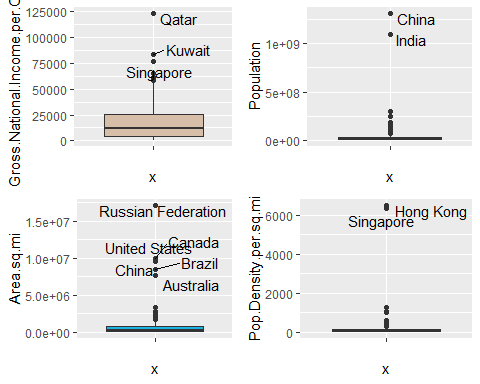
\includegraphics{DS6050.FinalProject.Bender_files/figure-latex/unnamed-chunk-27-1.pdf}

\begin{Shaded}
\begin{Highlighting}[]
\KeywordTok{grid.arrange}\NormalTok{(g5, g6, g7, g8, }\DataTypeTok{nrow =} \DecValTok{2}\NormalTok{)}
\end{Highlighting}
\end{Shaded}

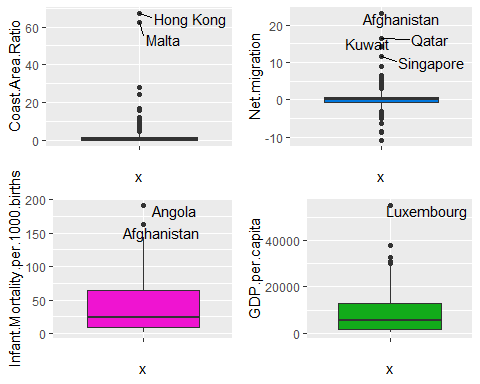
\includegraphics{DS6050.FinalProject.Bender_files/figure-latex/unnamed-chunk-27-2.pdf}

\begin{Shaded}
\begin{Highlighting}[]
\KeywordTok{grid.arrange}\NormalTok{(g9, g10, g11, g12, }\DataTypeTok{nrow =} \DecValTok{2}\NormalTok{)}
\end{Highlighting}
\end{Shaded}

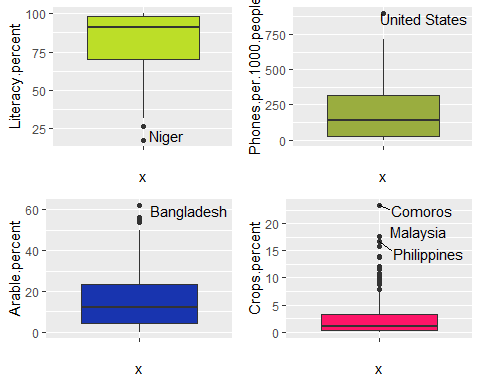
\includegraphics{DS6050.FinalProject.Bender_files/figure-latex/unnamed-chunk-27-3.pdf}

\begin{Shaded}
\begin{Highlighting}[]
\KeywordTok{grid.arrange}\NormalTok{(g13, g14, g15, }\DataTypeTok{nrow =} \DecValTok{2}\NormalTok{)}
\end{Highlighting}
\end{Shaded}

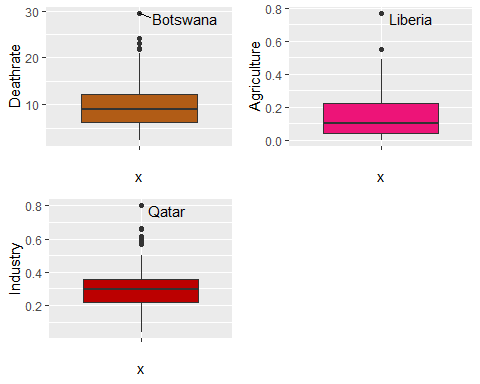
\includegraphics{DS6050.FinalProject.Bender_files/figure-latex/unnamed-chunk-27-4.pdf}

These boxplots (representing all of the features that contain outliers
based on z-score) clearly show a good story into the data. All of the
findings make sense with what we would expect and accessible layout the
distributions of the features as well as label the outlier countries.
The removal of outliers is something to take seriously. It could have
big negative ramifications if you remove outliers without justification.
Since all of the outliers here represent actual conditions out in the
world and are not based on data input error, I am going to make the
careful decision to leave them all in the dataset. This is an assumption
that will be marked. I will pay particular attention to output result
with these in mind. However, I fully expect that the presence of these
data points won't affect our analysis to a grand extent.

Also, since we don't have very many observations, once we scale our
data, outliers now may not remain outliers. Lastly, once more data is
collected (such as with the other countries in the world), it's possible
outliers won't be outliers anymore.

Let's do some more exploratory visualizations to get a sense of
relationships between variables.

\begin{Shaded}
\begin{Highlighting}[]
\NormalTok{r1 <-}\StringTok{ }\KeywordTok{ggplot}\NormalTok{(world_df, }\KeywordTok{aes}\NormalTok{(Region, Happiness.Score))}

\CommentTok{#show region names}
\KeywordTok{levels}\NormalTok{(world_df}\OperatorTok{$}\NormalTok{Region)}
\end{Highlighting}
\end{Shaded}

\begin{verbatim}
##  [1] "Australia and New Zealand"       "Central and Eastern Europe"     
##  [3] "Eastern Asia"                    "Latin America and Caribbean"    
##  [5] "Middle East and Northern Africa" "North America"                  
##  [7] "Southeastern Asia"               "Southern Asia"                  
##  [9] "Sub-Saharan Africa"              "Western Europe"
\end{verbatim}

\begin{Shaded}
\begin{Highlighting}[]
\CommentTok{#abbreviate region names to make graph more legible}
\NormalTok{reg_abbr <-}\StringTok{ }\KeywordTok{c}\NormalTok{(}\StringTok{"Australia and New Zealand"}\NormalTok{ =}\StringTok{ "Aus&NZ"}\NormalTok{, }\StringTok{"Central and Eastern Europe"}\NormalTok{ =}\StringTok{ "Cen.E Eur"}\NormalTok{,}\StringTok{"Eastern Asia"}\NormalTok{ =}\StringTok{ "E. Asia"}\NormalTok{, }\StringTok{"Latin America and Caribbean"}\NormalTok{ =}\StringTok{ "LatCari"}\NormalTok{, }\StringTok{"Middle East and Northern Africa"}\NormalTok{ =}\StringTok{ "MENA"}\NormalTok{, }\StringTok{"North America"}\NormalTok{ =}\StringTok{ "N. Amer."}\NormalTok{, }\StringTok{"Southeastern Asia"}\NormalTok{ =}\StringTok{ "SE. Asia"}\NormalTok{, }\StringTok{"Southern Asia"}\NormalTok{ =}\StringTok{ "S. Asia"}\NormalTok{, }\StringTok{"Sub-Saharan Africa"}\NormalTok{ =}\StringTok{ "S-S.Africa"}\NormalTok{, }\StringTok{"Western Europe"}\NormalTok{ =}\StringTok{ "W. Eur."}\NormalTok{)}

\CommentTok{#plot dotplot to show distribution}
\NormalTok{r1 }\OperatorTok{+}\StringTok{ }\KeywordTok{geom_dotplot}\NormalTok{(}\DataTypeTok{binaxis =} \StringTok{"y"}\NormalTok{, }\DataTypeTok{stackdir =} \StringTok{"center"}\NormalTok{, }\DataTypeTok{binwidth =} \FloatTok{0.1}\NormalTok{, }\DataTypeTok{fill =} \StringTok{"#1995AD"}\NormalTok{) }\OperatorTok{+}\StringTok{ }\KeywordTok{scale_x_discrete}\NormalTok{(}\DataTypeTok{labels =}\NormalTok{ reg_abbr) }\OperatorTok{+}\StringTok{ }\KeywordTok{ggtitle}\NormalTok{(}\StringTok{"Happiness Scores by Region"}\NormalTok{)}
\end{Highlighting}
\end{Shaded}

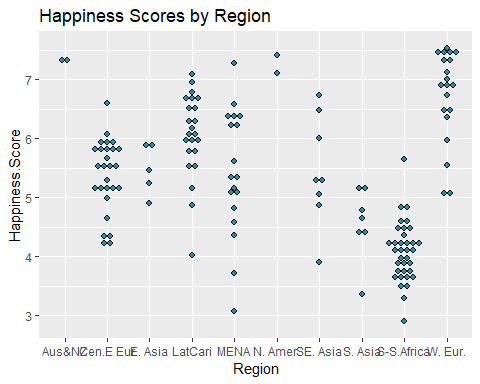
\includegraphics{DS6050.FinalProject.Bender_files/figure-latex/unnamed-chunk-28-1.pdf}
This dot plot nicely shows some distribution of happiness scores by
region. You can see some regions such as the Middle East and North
Africa have a large varaince. For example, there is a country with a
happiness score of just above 3, but there is also a country with a
happiness score of over 7. Also, you can see that the regions North
America and Australia \& NZ only have two members each.

Because the variance within regions is high and some regions only have a
few members, I anticipate my eventual classification of region may be
difficult. I can try to combat this with a few methods such as
stratified sampling, sampling with replacement, and k-fold cross
validation. We will see how it turns out!


\end{document}
